\documentclass[12pt]{report} % Use between book, article, beamer (presentation) etc...
%\documentclass[b5paper,12pt,twoside,openright]{report}
%\documentclass[a4paper,twoside,12pt]{report} % twoside command if using two sided, openright if needed
\usepackage[T1]{fontenc}
\usepackage[utf8]{inputenc} % This defines the font-encoding you prefer to use
\usepackage[norsk,UKenglish]{babel} %\selectlanguage{norsk}
\usepackage[a4paper, left=2cm, right=2cm]{geometry} % Setting margins on the paper - left=2cm, right=2cm, top=2cm, bottom=2cm
\usepackage{times} % Times new Roman
\usepackage{graphicx} % Adding grapichs
\usepackage{subcaption} % For subfigures
\usepackage{amsmath,amssymb,amsfonts} % For writing math more advanced than quadratic equations
\usepackage{mathtools} % For writing math more advanced than quadratic equations
\usepackage{wrapfig} % For adding figures next to each other
\usepackage{listings} % List of figures, tables, and custom made 
\usepackage{tcolorbox} % Colorbox for drawing
\usepackage{tikz} % Drawings
\usepackage{pdfpages} % For .pdf files
\usepackage{float} % Make graphics float if necessary
\usepackage{parskip} % Skip a line when pressing enter
\usepackage{siunitx} % SI units
\usepackage{makecell} % Make subcells
\usepackage{csquotes} % Quotes
\usepackage{enumitem} % Itemize numerical or dots

% Algoritmer
% ``listings'' package settings
\definecolor{dkgreen}{rgb}{0,0.6,0}
\definecolor{gray}{rgb}{0.5,0.5,0.5}
\definecolor{pink}{rgb}{0.63, 0.13, 0.94}
\lstset{language=Matlab, 
	keywords={break, case, catch, continue,else,elseif,end,for,function,
		global,if,otherwise,persistent,return,switch,try,while},
	basicstyle=\ttfamily,
	keywordstyle=\color{blue},
	commentstyle=\color{dkgreen},
	stringstyle=\color{pink},
	numbers=left,
	breaklines=true,
	numberstyle=\tiny\color{gray},
	stepnumber=1,
	numbersep=10pt,
	backgroundcolor=\color{white},
	tabsize=4,
	showspaces=false,
	showstringspaces=false,
    inputencoding=utf8}
\renewcommand{\lstlistingname}{Algorithm}% Listing -> Algorithm
\renewcommand*{\lstlistlistingname}{List of Algorithms}

% BIBLATEX
\usepackage[style=authoryear]{biblatex}
\addbibresource{sources.bib}
\renewcommand*{\nameyeardelim}{\addcomma\space} % Adding a comma

\NewBibliographyString{available}
\DefineBibliographyStrings{english}{available = {Available:}}
\DeclareFieldFormat{url}{\bibstring{available}\addcolon\space\url{#1}}
\DeclareFieldFormat{urldate}{\addcomma\space(Acsessed:\space#1)}

%%%%%%%%%%%%%%%%%%%%%


% Header and footer
\usepackage{fancyhdr}
\pagestyle{fancy}
\fancyhead{}
\fancyfoot{}
\fancyhead[L]{\slshape \oppgavetittel}
\fancyhead[R]{\slshape \rightmark}
\fancyfoot[C]{\thepage}
\setlength{\headheight}{15pt} % ...at least 14.49998 pt

\usepackage[colorlinks=true, pdfstartview=FitV,
linkcolor=black, citecolor=black, urlcolor=blue]{hyperref} % Color when making a reference.

% Hurtigtaster 
\newcommand{\bredde}{0.8\textwidth}
\newcommand{\oppgavetittel}{Tekna Student \LaTeX{} \today}
\newcommand{\kilde}{Bibliography}
\newcommand{\navn}{John Doe}
\newcommand{\supervisor}{Leif Andreas Hirsti}


%\includeonly{enumerate} % Faster compile

\begin{document}
\pagenumbering{Alph}

\begin{titlepage}
    
\includepdf[pages=1-]{FirstPage.pdf}
	\thispagestyle{plain}	
\includegraphics[width=0.3\textwidth]{hovedlogo.png}
	\begin{center}
		\vspace*{1cm}
		\LaTeX\space for Tekna medlemmer \\
		Introkurs\\[5cm]
	\end{center}		
		%\rule{\textwidth}{0.1cm}
		\huge{\oppgavetittel}\\
		%\rule{\textwidth}{0.1cm}
		\\[1cm]
		
		\Large{\textbf{\navn}}\\
		\vfill

		\normalsize{Master of Science in Industrial Cybernetics\\
		Submission date: \today\\
		Supervisor: \supervisor, ITK\\[1cm]
		Norwegian University of Science and Technology\\
		Department of Engineering Cybernetics}
	
	\newpage\null\thispagestyle{empty}\newpage % Custom made title page
\end{titlepage}



\pagenumbering{Roman}
\thispagestyle{plain}
\phantomsection
\addcontentsline{toc}{chapter}{Abstract}
\begin{abstract}
This course will show you how to write technical documents in \LaTeX.

This will not show how to write a master thesis.  
\end{abstract}



\selectlanguage{norsk}
\phantomsection
\addcontentsline{toc}{chapter}{Sammendrag}
\begin{abstract}
\setcounter{page}{2}
Dette kurset vil ta for seg den tekniske delen ved å skrive i \LaTeX.

Det vil ikke bli vist hvordan man skriver en masteroppgave.
\end{abstract}
\selectlanguage{UKenglish}


\newpage
\setcounter{page}{3}
\phantomsection
\addcontentsline{toc}{chapter}{Preface}
	\section*{Preface}
This is something
\thispagestyle{empty}


\tableofcontents
\newpage
\phantomsection
\addcontentsline{toc}{chapter}{List of figures}
\listoffigures

\newpage
\phantomsection
\addcontentsline{toc}{chapter}{List of tables}
\listoftables

\newpage
\phantomsection
\addcontentsline{toc}{chapter}{List of Algorithms}
\lstlistoflistings 

\cleardoublepage

\pagenumbering{arabic} 
\setcounter{page}{1}
\newpage\null\thispagestyle{empty}\newpage

\chapter{History}
Welcome to \LaTeX{} course for Tekna Student \today.

\section{1985}
\begin{quote}
    \textit{LaTeX, software used for typesetting technical documents. LaTeX is a free software package created in 1985 by the American computer scientist Leslie Lamport as an addition to the TeX typesetting system. LaTeX was created to make it easier to produce general-purpose books and articles within TeX.} -- \cite{LatexHistory}
\end{quote}

\subsection{\LaTeX{} mostly used today}
Most are in academia, not much in corporations. Corporations use Microsoft with extensions. 

\subsection{Writing subsections}
Here is a subsection.

\subsubsection{Subsubsection}
Here  is subsubsection.



\chapter{Equations}

This chapter we will lock at how to write equations. Take a look at equation \ref{determinat}.

\section{Integral}
\begin{align}
    &\int_{x=0}^3 x^2 + 3  \, dx\   \\
    &\left[\frac{1}{3}x^3 + 3x\right]_{x=0}^3 \\
    &\left[\frac{1}{3}3^3 + 3\cdot3\right] \\
    &= \underline{\underline{18}}
\end{align}

\section{Subequations}
\begin{subequations}
\begin{align}
    x&=Ax + Bu \\
    y&=Cx + Du
\end{align}
\end{subequations}

\section{Matrix}


\begin{align}
	\dot{\mathbf{x}} &= 
	\begin{bmatrix}
	1 & 2 \\
    3 & 4
	\end{bmatrix} \\
     \text{det } \dot{\mathbf{x}} &= \text{det } \begin{bmatrix}
       1 & 2 \\
        3 & 4  
     \end{bmatrix}\label{determinat}\\ 
     &= 1\cdot4 - 2\cdot3 = \underline{\underline{-2}}
\end{align}

\subsection{Larger matrix}
\begin{align}\label{AB matrix}
	\dot{\mathbf{x}} = 
	\begin{bmatrix}
	\dot{p_1}\\
	\dot{p_2}\\
	\vdots\\
	\dot{p_N}\\
	\dot{q_1}\\
	\dot{q_2}\\
	\vdots\\
	\dot{q_N}
	\end{bmatrix}
	&=
	\begin{bmatrix}
	0 & 0 & \ldots & 0 & -k_1 & 0 & \ldots & 0\\
	0 & 0 & \ldots & 0 & k_1 & -k_1 & \ldots & 0\\
	\vdots & \vdots &\ddots &\vdots &\vdots & \vdots & \ddots & \vdots \\
	0 & 0 & \ldots & 0 & 0 & 0 & \ldots & -k_1\\
	k_2 & -k_2 & \ldots & 0 & -f & 0 & \ldots & 0\\
	0 & k_2 & \ldots & 0 & 0 & -f & \ldots & 0\\
	\vdots & \vdots & \ddots & \vdots &\vdots &\vdots & \ddots & \vdots \\
	0 & 0 & \ldots & k_2 & 0 & 0 & \ldots & -f \\
	\end{bmatrix}
	\begin{bmatrix}
	p_1\\p_2\\\vdots\\p_N\\q_1\\q_2\\ \vdots\\q_N
	\end{bmatrix}\\
	&+ \begin{bmatrix}
	k_1 & 0\\ 0 & 0\\\vdots & \vdots\\ 0 & 0 \\ 0 & 0 \\ 0 & 0 \\\vdots & \vdots\\ 0 & -k_2
	\end{bmatrix} 
	\begin{bmatrix}
	q_{in} \\ p_{out}
	\end{bmatrix}
\end{align}

\section{With greek letters}
\begin{align}
	H(s) &= \frac{k_1\, k_2}{s^2 + d\,s + k_1\, k_2}\\
	H(s) &= \frac{k_1\, k_2}{s^2 + 2 \zeta \omega_0 s + \omega_0^2}\\
	\zeta &= \frac{d}{2\sqrt{k_1\, k_2}} \label{zeta 1}
\end{align}

\section{Laplace}
\begin{align}
	\mathcal{L}\{\dot{\mathbf{x}}\} &\Rightarrow s\mathbf{x}(s) = \mathbf{Ax}(s) + \mathbf{Bu}(s)\\
	\mathbf{x}(s) &= (s\mathbb{I} - \mathbf{A})^{-1} \mathbf{Bu}s\\
	\mathcal{L}\{\mathbf{y}\} &\Rightarrow \mathbf{y}(s) = \mathbf{Cx}(s) + \mathbf{Du}(s)\\
	\mathbf{y}(s)  &= \mathbf{C} (s\mathbb{I} - \mathbf{A})^{-1} \mathbf{Bu}(s) + \mathbf{Du}(s)\\
	\frac{\mathbf{y}}{\mathbf{u}}(s) &= \mathbf{H}(s) = \mathbf{C} (s\mathbb{I} - \mathbf{A})^{-1} \mathbf{B} + \mathbf{D}
\end{align}
\chapter{Tables}

How to write tabular, there are \textbf{many} ways to do so. See Table. \ref{tab:Tabletest}.

\begin{tabular}{l|c|r}
     Left & Center & Right \\ \hline
     once & more & time
\end{tabular}

\begin{table}[h]
    \centering
    \begin{tabular}{l|c|r} 
     Left & Center & Right \\ \hline
     More text & to see & the difference\\ 
     One extra & line for & fun
\end{tabular}
    \caption{Caption for tabular, will be added to list of tables}
    \label{tab:Tabletest}
\end{table}


\chapter{Lists}
When you want to itemize or enumerate.

\section{Itemize}
\begin{itemize}
    \item Item 1
    \item Item 2
    \begin{itemize}
        \item Sub item 1
        \item Sub item 2
    \end{itemize}
    \item Item 3
\end{itemize}

\section{Enumerate}
\begin{enumerate}
    \item Item 1
    \item Item 2
    \begin{enumerate}
        \item Sub item 1
        \item Sub item 2 
    \end{enumerate}
    \item Item 3
\end{enumerate}

\section{Combo}
\begin{enumerate}
    \item Item 1
    \item Item 2
    \begin{itemize}
        \item Sub item 1
        \item Sub item 2 
    \end{itemize}
    \item Item 3
\end{enumerate}

or 

\begin{itemize}
    \item Item 1
    \item Item 2
    \begin{enumerate}
        \item Sub item 1
        \item Sub item 2 
    \end{enumerate}
    \item Item 3
\end{itemize}

\chapter{Figures}

Adding figures is most likely necessary for a thesis.

\section{One figure}
\begin{figure}[h]
    \centering
    \caption{Tekna logo}
    
\includegraphics[width=0.8\textwidth]{hovedlogo.png}
    \label{fig:TeknaLogo}
\end{figure}

\newpage
\section{Sub figures}
\begin{figure}[h]
	\centering
	\begin{subfigure}[b]{0.35\textwidth}
		
\includegraphics[width=\textwidth]{hovedlogo.png}
		\caption{Tekna logo 1}
		\label{fig:TeknaLogo1}
	\end{subfigure}
	\qquad
	\begin{subfigure}[b]{0.35\textwidth}
		
\includegraphics[width=\textwidth]{hovedlogo.png}
		\caption{Tekna logo 2}
        \label{fig:TeknaLogo2}
	\end{subfigure}
	\caption{Two Tekna logos next to each other.}
    \label{fig:TeknaLogos}
\end{figure}

\chapter{Drawings}

Using package TikZ we will get a drawing instead of using Paint.


\section{Tank equation}
\begin{figure}[h]
    \centering
    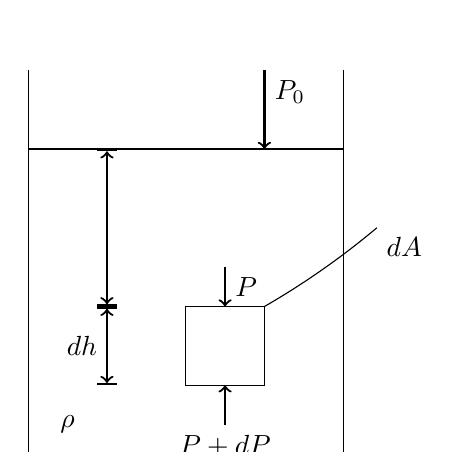
\begin{tikzpicture}
    \draw (0,0) rectangle (4,4);
    \draw (0,4) -- (0,5);
    \draw (4,4) -- (4,5);
    \draw[thick, <-] (3,4) -- (3,5) node[anchor=north west]{$P_0$};
    \draw (2,1) rectangle (3,2);
    \draw[thick, <-] (2.5,2) -- (2.5,2.5) node[anchor=north west]{$P$};
    \draw[thick, <-] (2.5,1) -- (2.5,0.5) node[anchor= north]{$P+dP$};
    \draw (0.5,0.5) node{$\rho$};
    \draw (3,2) arc (300:310:10cm) node[anchor=north west]{$dA$};
    \draw[thick, |<->|] (1,4) -- (1,2);
    \draw[thick, |<->|] (1,2) -- (1,1);
    \draw (1,1.5) node[anchor=east]{$dh$};
    \end{tikzpicture}
    \caption{Tank and pressure}
    \label{fig:tank}
\end{figure}

\newpage
\section{Ultrasound on objects}
\begin{figure}[h]
    \centering
    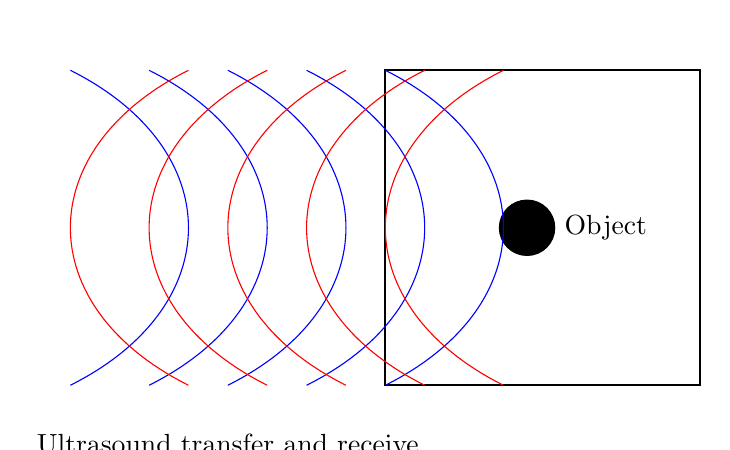
\begin{tikzpicture}
    \filldraw[color=black] (-2.2,0) circle (10pt) node[xshift=1cm] {Object};
    \draw[thick] (-4,-2) rectangle (0,2);
    \foreach \x in {4,5,6,7,8}
        \draw[color=blue] (-\x,2) .. controls (-\x+2,1) and (-\x+2,-1) .. (-\x,-2);
    \foreach \x in {2.5,3.5,4.5,5.5,6.5}
        \draw[color=red] (-\x,2) .. controls (-\x-2,1) and (-\x-2,-1) .. (-\x,-2);
    \draw (-6,-2.5) node[anchor=north] {Ultrasound transfer and receive};
    \end{tikzpicture}
    \caption{Ultrasound}
    \label{fig:Ultrasound}
\end{figure}

\newpage
\section{Control volumes}
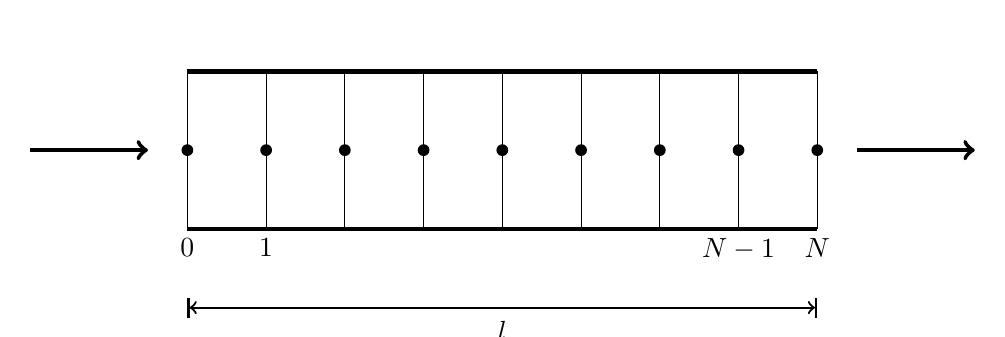
\begin{tikzpicture}
\foreach \x in {0,1}
   \draw (\x+2,2) rectangle (\x, 0) node[anchor=north] {$\x$};
\foreach \y in {2,3,4,5}   
   \draw (\y+2,2) rectangle (\y, 0);
\draw (7,2) rectangle (8,0) node[anchor=north] {$N$};
\draw (7,0) node[anchor=north] {$N-1$};
\draw[ultra thick] (0,0) -- (8,0);
\draw[ultra thick] (0,2) -- (8,2);
\draw[|<->|,thick] (0,-1) -- (8,-1) node[pos=0.5, yshift=-0.3cm]{$l$};
\draw[->, ultra thick] (-2,1) -- (-0.5,1);
\draw[->, ultra thick] (8.5,1) -- (10,1);
\foreach \n in {0,1,2,3,4,5,6,7,8}
  \node at (\n,1)[circle,fill,inner sep=1.5pt]{};
\end{tikzpicture}

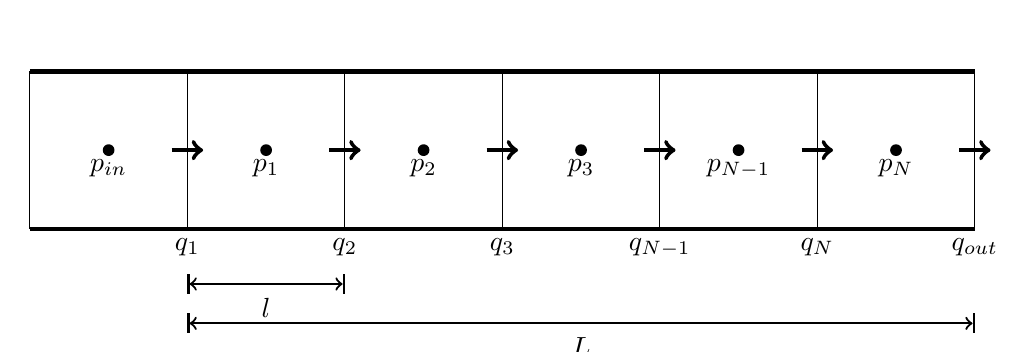
\begin{tikzpicture}
\foreach \x in {1,2,3}
   \draw (2*\x,2) rectangle (2*\x-2, 0) node[anchor=north] {$q_{\x}$};
\draw (8,2) rectangle (6, 0) node[anchor=north] {$q_{N-1}$};
\draw (10,2) rectangle (8, 0) node[anchor=north] {$q_{N}$};
\draw (8,2) rectangle (10,0) node[anchor=north] {$q_{out}$};
\draw (-2,2) rectangle (0,0);
\draw (-1,1) node[anchor=north] {$p_{in}$};
\draw[ultra thick] (-2,0) -- (10,0);
\draw[ultra thick] (-2,2) -- (10,2);
\draw[|<->|,thick] (0,-1.2) -- (10,-1.2) node[pos=0.5, yshift=-0.3cm]{$L$};
\draw[|<->|,thick] (0,-0.7) -- (2,-0.7) node[pos=0.5, yshift=-0.3cm]{$l$};
\foreach \n in {-1,1,3,5,7,9}
    \node at (\n,1)[circle,fill,inner sep=1.5pt]{};
\foreach \m in {1,2,3}
    \draw (2*\m-1,1) node[anchor=north] {$p_{\m}$};
\draw (7,1) node[anchor=north] {$p_{N-1}$};
\draw (9,1) node[anchor=north] {$p_{N}$};
\foreach \o in {0,2,4,6,8,10}
    \draw[->, ultra thick] (\o-0.2,1) -- (\o+0.2,1);
\end{tikzpicture}


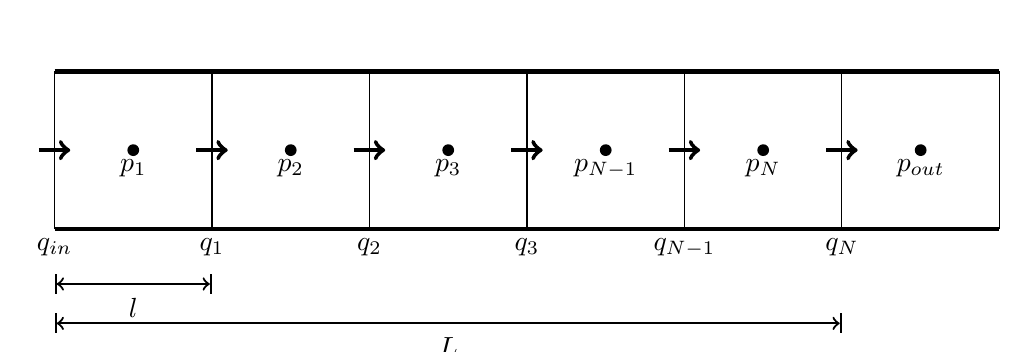
\begin{tikzpicture}
\foreach \x in {1,2,3}
   \draw (2*\x,2) rectangle (2*\x, 0) node[anchor=north] {$q_{\x}$};
\draw (8,2) rectangle (8, 0) node[anchor=north] {$q_{N-1}$};
\draw (10,2) rectangle (10, 0) node[anchor=north] {$q_{N}$};
\draw (0,0) node[anchor=north] {$q_{in}$};
\draw[ultra thick] (0,0) -- (12,0);
\draw[ultra thick] (0,2) -- (12,2);
\draw (11,1) node[anchor=north] {$p_{out}$};
\draw (0,0) -- (0,2);
\draw (12,0) -- (12,2);
\draw[|<->|,thick] (0,-1.2) -- (10,-1.2) node[pos=0.5, yshift=-0.3cm]{$L$};
\draw[|<->|,thick] (0,-0.7) -- (2,-0.7) node[pos=0.5, yshift=-0.3cm]{$l$};
\foreach \n in {1,3,5,7,9,11}
    \node at (\n,1)[circle,fill,inner sep=1.5pt]{};
\foreach \m in {1,2,3}
    \draw (2*\m-1,1) node[anchor=north] {$p_{\m}$};
\foreach \o in {0,2,4,6,8,10}
    \draw[->, ultra thick] (\o-0.2,1) -- (\o+0.2,1);
\draw (7,1) node[anchor=north] {$p_{N-1}$};
\draw (9,1) node[anchor=north] {$p_{N}$};
\end{tikzpicture}

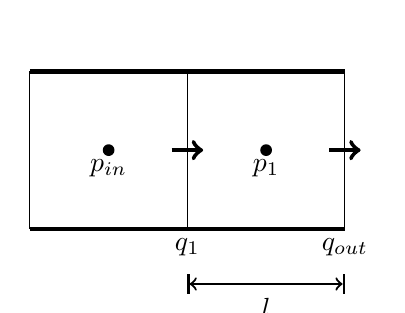
\begin{tikzpicture}
\draw (0,2) rectangle (2, 0) node[anchor=north] {$q_{out}$};
\draw (0,2) rectangle (-2, 0);
\draw (0,0) node[anchor=north] {$q_{1}$};
\draw (-1,1) node[anchor=north] {$p_{in}$};
\draw[ultra thick] (-2,0) -- (2,0);
\draw[ultra thick] (-2,2) -- (2,2);
\draw[|<->|,thick] (0,-0.7) -- (2,-0.7) node[pos=0.5, yshift=-0.3cm]{$l$};
\foreach \n in {0,1}
    \node at (2*\n-1,1)[circle,fill,inner sep=1.5pt]{};
\foreach \m in {1}
    \draw (2*\m-1,1) node[anchor=north] {$p_{\m}$};
\foreach \o in {0,2}
    \draw[->, ultra thick] (\o-0.2,1) -- (\o+0.2,1);
\end{tikzpicture}


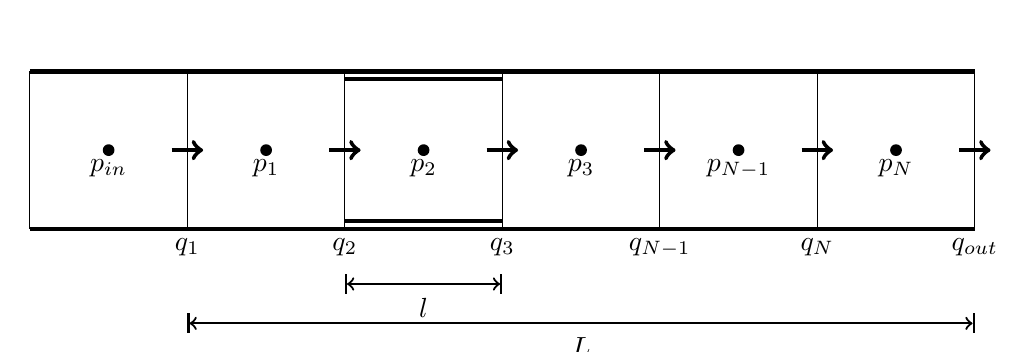
\begin{tikzpicture}
\foreach \x in {1,2,3}
   \draw (2*\x,2) rectangle (2*\x-2, 0) node[anchor=north] {$q_{\x}$};
\draw (8,2) rectangle (6, 0) node[anchor=north] {$q_{N-1}$};
\draw (10,2) rectangle (8, 0) node[anchor=north] {$q_{N}$};
\draw (8,2) rectangle (10,0) node[anchor=north] {$q_{out}$};
\draw (-2,2) rectangle (0,0);
\draw (-1,1) node[anchor=north] {$p_{in}$};
\draw[ultra thick] (-2,0) -- (10,0);
\draw[ultra thick] (-2,2) -- (10,2);
\draw[ultra thick] (4,0.1) -- (2,0.1);
\draw[ultra thick] (4,1.9) -- (2,1.9);
\draw[|<->|,thick] (0,-1.2) -- (10,-1.2) node[pos=0.5, yshift=-0.3cm]{$L$};
\draw[|<->|,thick] (4,-0.7) -- (2,-0.7) node[pos=0.5, yshift=-0.3cm]{$l$};
\foreach \n in {-1,1,3,5,7,9}
    \node at (\n,1)[circle,fill,inner sep=1.5pt]{};
\foreach \m in {1,2,3}
    \draw (2*\m-1,1) node[anchor=north] {$p_{\m}$};
\draw (7,1) node[anchor=north] {$p_{N-1}$};
\draw (9,1) node[anchor=north] {$p_{N}$};
\foreach \o in {0,2,4,6,8,10}
    \draw[->, ultra thick] (\o-0.2,1) -- (\o+0.2,1);
\end{tikzpicture}


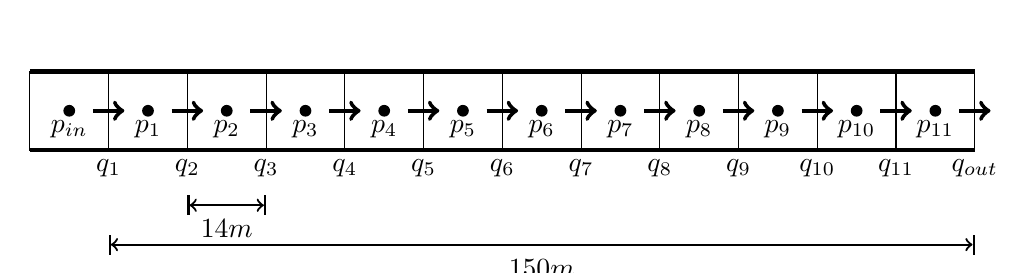
\begin{tikzpicture}
\foreach \x in {1,2,3,4,5,6,7,8,9,10,11}
   \draw (1*\x,1) rectangle (\x-1, 0) node[anchor=north] {$q_{\x}$};
\draw (10,1) rectangle (11,0) node[anchor=north] {$q_{out}$};
\draw (-1,1) rectangle (0,0);
\draw (-0.5,0.5) node[anchor=north] {$p_{in}$};
\draw[ultra thick] (-1,0) -- (11,0);
\draw[ultra thick] (-1,1) -- (11,1);
\draw[|<->|,thick] (0,-1.2) -- (11,-1.2) node[pos=0.5, yshift=-0.3cm]{$150 m$};
\draw[|<->|,thick] (1,-0.7) -- (2,-0.7) node[pos=0.5, yshift=-0.3cm]{$14 m$};
\foreach \n in {0,1,2,3,4,5,6,7,8,9,10,11}
    \node at (\n-0.5,0.5)[circle,fill,inner sep=1.5pt]{};
\foreach \m in {1,2,3,4,5,6,7,8,9,10,11}    
    \draw (\m-0.5,0.5) node[anchor=north] {$p_{\m}$};
\foreach \o in {0,1,2,3,4,5,6,7,8,9,10,11}
    \draw[->, ultra thick] (\o-0.2,0.5) -- (\o+0.2,0.5);
\end{tikzpicture}




\chapter{Links}

\section{Adding link}

Link to Tekna.no \href{https://www.tekna.no}{here}. 

Website: \href{https://www.overleaf.com/learn}{https://www.overleaf.com/learn}
\chapter{Algorithm}
Code can be added either written in \LaTeX{} or add the code from file.

\section{Written in \LaTeX}
\begin{lstlisting}[caption=MATLAB function Kalman filter,language=matlab,label=DKF algo]
function x_hat = KalmanFilter(u,y,KalmanData)
	persistent init A B C Q R P_ x_
		if isempty(init)
		init = 1; % Initialize the Kalman Filter
		[A,B,C,x_,P_,Q,R] = deal(KalmanData.A, KalmanData.B, KalmanData.C, KalmanData.x, KalmanData.P, KalmanData.Q, KalmanData.R);
		end
		L = (P_*C')*pinv(C*P_*C' + R); % Kalman gain
		x = x_ + L*(y-C*x_); % Update estimate with measurement y
		P = (eye(22)-L*C)*P_*(eye(22)-L*C)' + L*R*L'; % Compute error covariance for updated estimate
		x_ = A*x + B*u; % Project ahead
		P_ = A*P*A' + Q; % Predict error covariance
		x_hat = x;
end
\end{lstlisting}

\newpage
\section{From file}
\lstinputlisting[caption=Python program from a .py file.,language=python,firstnumber=14]{algorithm/HelpingCode.py}
%%%%% Kildehenvisning
\nocite{OverleafDocumentation}
\nocite{MasterThesis}
\phantomsection
\addcontentsline{toc}{chapter}{\kilde}
\printbibliography
\appendix
\newpage
\phantomsection
\addcontentsline{toc}{part}{Appendix}
\part*{Appendix}

\chapter{Nomenclature}
\begin{table}[h]
	\begin{tabular}{ll}
		$\beta$	& Bulk modulus\\
		$\rho$ 	& Density material, $\si{kg/m^3}$\\
		$A$		& Cross-section area, $\si{m^2}$\\
		$c$		& Speed of sound\\
		$d$		& Friction factor\\
		$f$		& Friction factor\\
		$g$		& Gravitational acceleration, $9,81 \si{m/s^2}$\\
		$H(s)$	& Transfer function\\
		$k$		& Constant\\
		$l$		& Length of pipesegment, $\si{m}$\\		
		$L$		& Length, $\si{m}$\\
		$\mathcal{L}$ & Laplace transformation\\
		$n$		& Number of nodes\\
		$\mathcal{O}$ & Observability\\
		$p$ 	& Pressure, $\si{Pa}$\\
		$q$		& Flow, $\si{m^3/s}$\\
		$r\_wax$	& Thickness wax, $\si{m}$\\
		$Z$		& Acoustic impedance, $\si{kg/m^2 s}$
	\end{tabular}
\end{table}

\chapter{Front page}
This is how UiA want you to write your frontpage \parencite{UiAThesis}.

\includepdf[pages=1-,scale=1]{FirstPage.pdf}






\end{document}
